%%%%(c)
%%%%(c)  This file is a portion of the source for the textbook
%%%%(c)
%%%%(c)    Abstract Algebra: Theory and Applications
%%%%(c)    Copyright 1997 by Thomas W. Judson
%%%%(c)
%%%%(c)  See the file COPYING.txt for copying conditions
%%%%(c)
%%%%(c)
\chap{Cyclic Groups}{cyclic}
 
The groups $\mathbb Z$ and ${\mathbb Z}_n$, which are among the most familiar and easily understood groups, are both examples of what are called cyclic groups.  In this chapter we will study the properties of cyclic groups and cyclic subgroups, which play a fundamental part in the classification of all abelian groups. 


\section{Cyclic Subgroups}

Often a subgroup will depend entirely on a single element of the group; that is, knowing that particular element will allow us to compute any other element in the subgroup. 

\begin{example}{Cyclic_Z3}
Suppose that we consider $3 \in {\mathbb Z}$ and look at all multiples (both positive and negative) of 3.  As a set, this is 
\[
3 {\mathbb Z} = \{ \ldots, -3, 0, 3, 6, \ldots \}.
\]
It is easy to see that $3 {\mathbb Z}$ is a subgroup of the integers.  This subgroup is completely determined by the element 3 since we can obtain all of the other elements of the group by taking multiples of 3.  Every element in the subgroup is ``generated'' by 3. 
\end{example}

\begin{example}{Cyclic_2^n}
If $H = \{ 2^n : n \in {\mathbb Z} \}$, then $H$ is a subgroup of the multiplicative group of nonzero rational numbers, ${\mathbb Q}^*$.  If $a = 2^m$ and $b = 2^n$ are in $H$, then $ab^{-1} = 2^m 2^{-n} = 2^{m-n}$ is also in $H$.  By Proposition~\ref{groups:subgroup_prop}, $H$ is a subgroup of ${\mathbb Q}^*$ determined by the element 2. 
\end{example}

\begin{theorem}
Let $G$ be a group and $a$ be any element in $G$.  Then the set
\[
\langle a \rangle  = \{ a^k : k \in {\mathbb Z} \}\label{generatedby}
\]
is a subgroup of $G$.  Furthermore, $\langle a \rangle$ is the smallest subgroup of $G$ that contains~$a$. 
\end{theorem}
 
 
\begin{proof}
The identity is in $\langle a \rangle $ since $a^0 = e$. If $g$ and
$h$ are any two elements in $\langle a \rangle $, then by the
definition of $\langle a \rangle$ we can write $g = a^m$ and $h = a^n$
for some integers $m$ and $n$. So $gh = a^m a^n = a^{m+n}$ is again in
$\langle a \rangle $. Finally, if $g = a^n$ in $\langle a \rangle $,
then the inverse $g^{-1} = a^{-n}$ is also in $\langle a \rangle $.
Clearly, any subgroup $H$ of $G$ containing $a$ must contain all the
powers of $a$ by closure; hence, $H$ contains $\langle a \rangle $.
Therefore, $\langle a \rangle $ is the smallest subgroup of $G$
containing $a$. 
\end{proof}
 
 
\medskip
 
 
\noindent {\bf Remark.}
If we are using the ``+'' notation, as in the case of the integers under
addition, we write $\langle a \rangle  = \{ na : n \in {\mathbb Z} \}$.
 
 
\medskip
 
 
For $a \in G$, we call $\langle a \rangle $ the {\bfi cyclic
subgroup\/}\index{Subgroup!cyclic} generated by $a$. If $G$ contains
some element $a$ such that $G = \langle a \rangle $, then $G$ is a
{\bfi cyclic group}\index{Group!cyclic}. In this case $a$ is a {\bfi
generator\/}\index{Generator of a cyclic subgroup} of $G$.  If $a$ is an
element of a group $G$, we define the {\bfi order}\index{Element!order
of} of $a$ to be the smallest positive integer $n$ such that $a^n= e$,
and we write $|a| = n$\label{noteelementorder}. If there is no such
integer $n$, we say that the order of $a$ is infinite and  write $|a|
= \infty$ to denote the order of $a$.
 
 
\begin{example}{Cyclic_Z6}
Notice that a cyclic group can have more than a single
generator. Both 1 and 5 generate ${\mathbb Z}_6$; hence, ${\mathbb Z}_6$ is
a cyclic group. Not every element in a cyclic group is necessarily a
generator of the group. The order of $2 \in {\mathbb Z}_6$ is 3. The
cyclic subgroup generated by 2 is $\langle 2 \rangle  = \{ 0, 2, 4
\}$.  
\end{example}
 
 
The groups ${\mathbb Z}$ and ${\mathbb Z}_n$ are cyclic groups. The elements
1 and $-1$ are generators for ${\mathbb Z}$.  We can certainly generate
${\mathbb Z}_n$ with 1 although there may be other generators of ${\mathbb
Z}_n$, as in the case of ${\mathbb Z}_6$. 
 
 
\begin{example}{Cyclic_U9}
The group of units, $U(9)$, in ${\mathbb Z}_9$ is a cyclic group.  As a
set, $U(9)$ is $\{ 1, 2, 4, 5, 7, 8  \}$. The element 2 is a generator
for $U(9)$ since 
\begin{align*}
2^1 & = 2 \qquad 2^2 = 4 \\
2^3 & = 8 \qquad 2^4 = 7 \\
2^5 & =  5 \qquad 2^6 = 1.
\end{align*}
\end{example}
 
 
\begin{example}{Not_Cyclic_S3}
Not every group is a cyclic group.  Consider the symmetry group of an
equilateral triangle $S_3$.  The multiplication table for this group
is Table~\ref{S3_table}. The subgroups of $S_3$ are shown in
Figure~\ref{subgrpsS3}.  Notice that every subgroup is cyclic;
however, no single element generates the entire group.
\hspace*{1in}
\end{example}


\begin{figure}[htb] %Replaced figure with tikz figure - TWJ 5/6/2010
\begin{center}
\tikzpreface{cyclic_s3_subgroups}
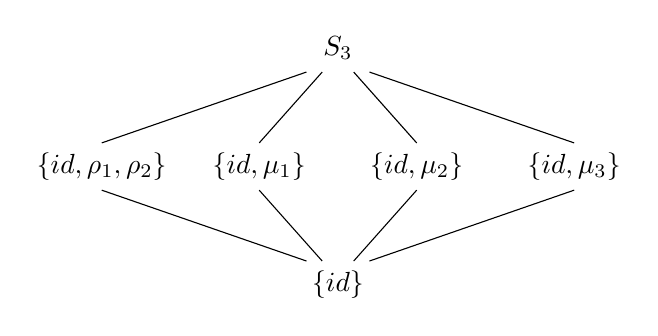
\begin{tikzpicture}[scale=1]

\draw  (0,0.3) -- (2.6,1.2);
\draw  (2,0.3) -- (2.8,1.2);
\draw  (4,0.3) -- (3.2,1.2);
\draw  (6,0.3) -- (3.4,1.2);

\draw  (0,-0.3) -- (2.6,-1.2);
\draw  (2,-0.3) -- (2.8,-1.2);
\draw  (4,-0.3) -- (3.2,-1.2);
\draw  (6,-0.3) -- (3.4,-1.2);

\node at (0, 0) {$\{  id, \rho_1, \rho_2\}$};
\node at (2, 0) {$\{  id, \mu_1\}$};
\node at (4, 0) {$\{  id, \mu_2 \}$};
\node at (6, 0) {$\{  id, \mu_3 \}$};
\node at (3, 1.5) {$S_3$};
\node at (3,-1.5) {$\{ id \}$};
\end{tikzpicture}
\end{center}
\caption{Subgroups of $S_3$}
\label{subgrpsS3}
\end{figure}
 
 
\begin{theorem}
Every cyclic group is abelian.
\end{theorem}
 
 
\begin{proof}
Let $G$ be a cyclic group and $a \in G$ be a generator for $G$. If
$g$ and $h$ are in $G$, then they can be written as powers of $a$,
say $g = a^r$ and $h = a^s$. Since
\[
g  h = a^r a^s = a^{r+s} = a^{s+r} = a^s a^r = h g,
\]
$G$ is abelian.
\end{proof}
 
 
 
\subsection*{Subgroups of Cyclic Groups}
 
 
We can ask some interesting questions about cyclic subgroups of a
group and subgroups of a cyclic group.  If $G$ is a group, which
subgroups of $G$ are cyclic? If $G$ is a cyclic group, what type of
subgroups does $G$ possess? 
 
 
 
\begin{theorem}
Every subgroup of a cyclic group is cyclic.
\end{theorem}
 
 
\begin{proof}
The main tools used in this proof are the division algorithm and the
Principle of Well-Ordering. Let $G$ be a cyclic group generated by $a$
and suppose that $H$ is a subgroup of $G$. If $H = \{ e \}$, then
trivially $H$ is cyclic. Suppose that $H$ contains some other element
$g$ distinct from the identity. Then $g$ can be written as
$a^n$ for some integer $n$. We can assume that $n > 0$. Let $m$ be the
smallest natural number such that $a^m \in H$. Such an $m$ exists by
the Principle of Well-Ordering.
 
 
We claim that $h = a^m$ is a generator for $H$.  We must show that
every $h' \in H$ can be written as a power of $h$. Since $h' \in H$
and $H$ is a subgroup of $G$, $h' = a^k$ for some positive integer
$k$. Using the division algorithm, we can find numbers $q$ and $r$
such that $k = mq +r$ where $0 \leq r < m$; hence,
\[
a^k = a^{mq +r} = (a^m)^q a^r = h^q a^r.
\]
So $a^r = a^k h^{-q}$. Since $a^k$ and $h^{-q}$ are in $H$, $a^r$ must
also be in $H$.  However, $m$ was the smallest positive number such that
$a^m$ was in $H$; consequently, $r=0$ and so $k=mq$. Therefore, 
\[
h' = a^k = a^{mq} =  h^q
\]
and $H$ is generated by $h$.
\end{proof}
 
 
\begin{corollary}
The subgroups of ${\mathbb Z}$ are exactly $n{\mathbb Z}$ for $n = 0, 1, 2,
\ldots$. 
\end{corollary}
 
 
\begin{proposition}\label{Cyclic_subgrp_order}
Let $G$ be a cyclic group of order $n$ and suppose that $a$ is a
generator for  $G$. Then $a^k=e$ if and only if $n$ divides $k$.
\end{proposition}
 
 
\begin{proof}
First suppose that $a^k=e$. By the division algorithm, $k = nq + r$
where $0 \leq r < n$; hence, 
\[
e = a^k = a^{nq + r} = a^{nq} a^r = e a^r = a^r.
\]
Since the smallest positive integer $m$ such that $a^m = e$ is $n$, $r
= 0$.
 
 
Conversely, if $n$ divides $k$, then $k=ns$ for some integer $s$.
Consequently, 
\[
a^k = a^{ns} = (a^n)^s = e^s = e.
\]
\end{proof}
 
 
\begin{theorem}
Let $G$ be a cyclic group of order $n$ and suppose that $a \in G$ is a
generator of the group.  If $b = a^k$, then the order of $b$ is $n
/d$, where $d = \gcd(k,n)$. 
\end{theorem}
 
 
\begin{proof}
We wish to find the smallest integer $m$ such that $e = b^m = a^{km}$.
By Proposition~\ref{Cyclic_subgrp_order}, this is the smallest integer $m$ such that
$n$ divides $km$ or, equivalently, $n/d$ divides $m(k/d)$.  Since $d$ is
the greatest common divisor of $n$ and $k$, $n/d$ and $k/d$ are
relatively prime. Hence, for $n/d$ to divide $m(k/d)$ it must divide
$m$.  The smallest such $m$ is $n/d$. 
\end{proof}
 
 
\begin{corollary}
The generators of ${\mathbb Z}_n$ are the integers $r$ such that $1 \leq
r < n$ and $\gcd(r,n) =  1$. 
\end{corollary}
 
 
\begin{example}{Cyclic_Z16}
Let us examine the group ${\mathbb Z}_{16}$.  The numbers 1, 3, 5, 7, 9,
11, 13, and 15 are the elements of ${\mathbb Z}_{16}$ that are relatively
prime to 16.  Each of these elements generates ${\mathbb Z}_{16}$. For
example, 
\begin{alignat*}{3}
1 \cdot 9  & =  9  & \qquad 2 \cdot 9  & = 2  & \qquad 3 \cdot 9  & = 11 \\
4 \cdot 9  & =  4  & \qquad 5 \cdot 9  & = 13 & \qquad	6 \cdot 9 & = 6  \\
7 \cdot 9  & =  15 & \qquad 8 \cdot 9  & = 8  & \qquad	9 \cdot 9 &  = 1  \\
10 \cdot 9 & =  10 & \qquad 11 \cdot 9 & = 3  & \qquad	12 \cdot 9 &  = 12 \\
13 \cdot 9 & =  5 &  \qquad 14 \cdot 9 & = 14 &  \qquad	15 \cdot 9 & = 7.
\end{alignat*}
\end{example}
 
 
%\section{The Group ${\mathbb C}^\ast$}

\section{The Multiplicative Group of Complex Numbers}
 
 
The {\bfi complex numbers} are defined as
\[
{\mathbb C} = \{ a + bi : a, b \in {\mathbb R} \},
\]
where $i^2 = -1$.  If $z=a+bi$, then $a$ is the {\bfi real part} of $z$
and $b$ is the {\bfi imaginary part} of $z$. 
 
 
To add two complex numbers $z=a+bi$ and $w= c+di$, we just
add the corresponding real and imaginary parts:
\[
z+w=(a + bi ) + (c + di)  =  (a+c) + (b+d)i.
\]
Remembering that $i^2 = -1$,  we multiply complex numbers just like
polynomials. The product of $z$ and $w$ is 
\[
(a + bi )(c + di)  =   ac + bdi^2 + adi + bci =  (ac -bd) +
(ad + bc)i.
\]
 
 
Every nonzero complex number $z = a +bi$ has a multiplicative inverse;
that is, there exists a $z^{-1} \in {\mathbb C}^\ast$ such that $z z^{-1}
= z^{-1} z = 1$. If $z = a + bi$, then 
\[
z^{-1} = \frac{a-bi}{ a^2 + b^2  }.
\]
The {\bfi complex conjugate}\index{Conjugate, complex} of a complex
number $z = a +bi$ is defined to be $\overline{z} = a-bi$.  The {\bfi
absolute value} or {\bfi modulus} of  $z = a +bi$  is $|z| =
\sqrt{a^2+b^2}$.  
 
 
\begin{example}{complex_add}
Let $z = 2 + 3i$ and $w = 1-2i$. Then
\[
z + w = (2 + 3i)+( 1-2i ) = 3 +i
\]
and
\[
z  w = (2 + 3i)( 1-2i ) = 8-i.
\]
Also,
\begin{align*}
z^{-1} & = \frac{2}{13} - \frac{3}{13}i \\
|z| & = \sqrt{13} \\
\overline{z} & = 2-3i.
\end{align*}
\end{example}
 
\begin{figure}[hbt]  %Replaced figure with tikz figure - TWJ 5/6/2010
\begin{center}
\tikzpreface{cyclic_complex_rectangular}
\begin{tikzpicture}[scale=0.5]

\draw [->]  (0,-5) -- (0,5);
\draw  [->] (-8,0) -- (8,0);
\node [right] at (0,5) {$y$};
\node [below] at (8,0) {$x$};
\node [below] at (0.5,0) {$0$};

\filldraw[fill=black, draw=black] (2,3) circle (0.05cm);
\node [right] at (2,3) {$z_1 = 2 + 3i$};

\filldraw[fill=black, draw=black] (-3,2) circle (0.05cm);
\node [left] at (-3, 2) {$z_3 = -3 + 2i$};

\filldraw[fill=black, draw=black] (1,-2) circle (0.05cm);
\node [right] at (1, -2) {$z_2 = 1 -  2i$};

\end{tikzpicture}
\end{center}
\caption{Rectangular coordinates of a complex number}
\label{rectcoord}
\end{figure}
 
 
There are several ways of graphically representing complex numbers. We
can represent a complex number $z = a +bi$ as an ordered pair on the
$xy$ plane where $a$ is the $x$ (or real) coordinate and $b$ is the $y$
(or imaginary) coordinate. This is called the {\bfi rectangular} or
{\bfi Cartesian} representation. The rectangular representations of
$z_1 = 2 + 3i$, $z_2 = 1 - 2i$, and $z_3 = - 3 + 2i$ are depicted in
Figure~\ref{rectcoord}.
 
 
\begin{figure}[htb]
\begin{center}
\tikzpreface{cyclic_complex_polar}
\begin{tikzpicture}[scale=0.5] %Replaced figure with tikz figure - TWJ 5/6/2010

\draw [->]  (0,-5) -- (0,5);
\draw  [->] (-8,0) -- (8,0);
\node [right] at (0,5) {$y$};
\node [below] at (8,0) {$x$};
\node [below] at (0.5,0) {$0$};

\draw (0,0) -- (35:6);
\draw (2,0) arc (0:35:2);

\filldraw[fill=black, draw=black] (35:6) circle (0.05cm);
\node [right] at (35:6) {$a + bi$};
\node [above] at (35:3) {$r$};
\node [right] at (17:2) {$\theta$};

\end{tikzpicture}

\end{center}
\caption{Polar coordinates of a complex number}
\label{polarcoord}
\end{figure}
 
 
Nonzero complex numbers can also be represented using {\bfi polar
coordinates}.  To specify  any nonzero point on the plane, it suffices
to give an angle $\theta$ from the positive $x$ axis in the
counterclockwise direction and a distance $r$ from the origin, as in 
Figure~\ref{polarcoord}. We can see that 
\[
z = a + bi = r( \cos \theta + i \sin \theta).
\]
Hence,
\[
r = |z| = \sqrt{a^2+b^2}
\]
and
\begin{align*}
a & = r \cos \theta \\
b & = r \sin \theta.
\end{align*}
We sometimes abbreviate $r( \cos \theta + i \sin \theta)$ as $r \cis
\theta$\label{cosisin}.  To assure that the representation of $z$ is 
well-defined, we also require that $0^{\circ} \leq \theta <
360^{\circ}$.  If the measurement is in radians, then $0 \leq \theta <
2 \pi$. 
 
\begin{example}{polar}
Suppose that $z = 2 \cis  60^{\circ}$. Then
\[
a  =  2 \cos 60^{\circ}  =   1
\]
and
\[
b  =  2 \sin 60^{\circ}  =  \sqrt{3}.
\]
Hence, the rectangular representation is $z = 1+\sqrt{3}\, i$.
 
 
Conversely, if we are given a rectangular representation of a complex
number, it is often useful to know the number's polar representation.
If $z = 3 \sqrt{2} - 3 \sqrt{2}\, i$, then 
\[
r = \sqrt{a^2 + b^2} = \sqrt{36 } = 6
\]
and
\[
\theta = \arctan \left( \frac{b}{a} \right) = \arctan( - 1) =
315^{\circ},
\]
so $3 \sqrt{2} - 3 \sqrt{2}\, i=6 \cis  315^{\circ}$.
\end{example}
 
 
The polar representation of a complex number makes it easy to find
products and powers of complex numbers.  The proof of the following
proposition is straightforward and is left as an exercise.
 
 
\begin{proposition}\label{polar_mult}
Let $z = r \cis \theta$ and $w = s \cis \phi$
be two nonzero complex numbers. Then 
\[
zw = r s \cis( \theta + \phi).
\]
\end{proposition}
 
 
\begin{example}{polar_mult}
If $z =  3 \cis( \pi / 3 )$ and $w = 2 \cis(\pi / 6 )$, then $zw = 6
\cis( \pi / 2 ) = 6i$.  
\end{example}
 
 
\begin{theorem}[DeMoivre]\index{DeMoivre's Theorem}
Let $z = r \cis  \theta$ be a nonzero complex number. Then 
\[
[r \cis \theta  ]^n
=
r^n \cis( n \theta)
\]
for $n = 1, 2, \ldots$.
\end{theorem}
 
 
\begin{proof}
We will use induction on $n$. For $n = 1$ the theorem is trivial.
Assume that the theorem is true for all $k$ such that $1  \leq k \leq
n$. Then 
\begin{align*}
z^{n+1} & = z^n z \\
& =
r^n( \cos  n \theta + i \sin n \theta ) r( \cos \theta + i
\sin \theta ) \\
& =
r^{n+1} [( \cos n \theta \cos \theta - \sin n \theta \sin
\theta )
 + i ( \sin n \theta \cos \theta + \cos n \theta \sin \theta
)] \\
& =
r^{n+1} [ \cos( n \theta + \theta) + i \sin( n \theta +
\theta) ] \\
& =
r^{n+1} [ \cos( n +1) \theta + i \sin( n+1) \theta  ].
\end{align*}
\end{proof}
 
 
\begin{example}{DeMoivre}
Suppose that $z= 1+i$ and we wish to compute $z^{10}$. Rather than
computing $(1+i)^{10}$ directly, it is much easier to switch to polar
coordinates and calculate $z^{10}$ using DeMoivre's Theorem:
\begin{align*}
z^{10}
& =
(1+i)^{10} \\
& =
\left( \sqrt{2} \cis \left( \frac{\pi }{4} \right)
\right)^{10} \\
& =
( \sqrt{2}\, )^{10} \cis \left( \frac{5\pi }{2} \right)
\\
& =
32  \cis \left( \frac{\pi }{2} \right) \\
& = 32i.
\end{align*}
\end{example}
 
 
\subsection*{The Circle Group and the Roots of Unity }
 
 
The multiplicative group of the complex numbers, ${\mathbb C}^*$,
possesses some interesting subgroups.  Whereas ${\mathbb Q}^*$ and ${\mathbb
R}^*$ have no interesting subgroups of finite order, ${\mathbb C}^*$ has 
many. We first consider the {\bfi circle group}\index{Group!circle}, 
\[
{\mathbb T}\label{notecirclegroup} = \{ z \in {\mathbb C} : |z| = 1 \}.
\]
The following proposition is a direct result of Proposition~\ref{polar_mult}.
 
 
\begin{proposition}
The circle group is a subgroup of  ${\mathbb C}^*$.
\end{proposition}
 
 
Although the circle group has infinite order, it has many interesting 
finite subgroups. Suppose that $H = \{ 1, -1, i, -i \}$. Then $H$ is a
subgroup of the circle group. Also, $1$, $-1$, $i$, and $-i$ are
exactly those complex numbers that satisfy the equation $z^4=1$. 
The complex numbers satisfying the equation $z^n=1$ are called
the {\bfi nth roots of unity}\index{$n$th root of unity}. 
 
 
\begin{theorem}
If $z^n = 1$, then the $n$th roots of unity are
\[
z = \cis\left( \frac{2 k \pi}{n } \right),
\]
where $k = 0, 1, \ldots, n-1$. Furthermore, the $n$th roots of unity
form a cyclic subgroup of\/ ${\mathbb T}$ of order $n$. 
\end{theorem}
 
 
\begin{proof}
By DeMoivre's Theorem,
\[
z^n = \cis \left( n \frac{2 k \pi}{n } \right) =
\cis( 2 k \pi ) = 1.
\]
The $z$'s are distinct since the numbers $2 k \pi /n$ are all
distinct and are greater than or equal to 0 but less than $2 \pi$.
The fact that these are all of the roots of the equation $z^n=1$
follows from from Corollary~\ref{poly:zeros_corollary}, which
states that a polynomial of degree $n$ can have at most $n$ roots.  We
will leave the proof that the $n$th roots of unity form a cyclic
subgroup of ${\mathbb T}$ as an exercise.
\end{proof}
 
 
\medskip
 
 
A generator for the group of the $n$th roots of unity is called a
{\bfi primitive nth root of unity}\index{Primitive $n$th root of
unity}. 
 
 
\begin{example}{roots_unity}
The 8th roots of unity can be represented as
eight equally spaced points on the unit circle (Figure~\ref{rtsunity}).  The
primitive 8th roots of unity are
\begin{align*}
\omega & = \frac{\sqrt{2}}{2}  + \frac{\sqrt{2}}{2} i \\
\omega^3 & = -\frac{\sqrt{2}}{2}  + \frac{\sqrt{2}}{2} i \\
\omega^5 & = -\frac{\sqrt{2}}{2}  - \frac{\sqrt{2}}{2} i \\
\omega^7 & = \frac{\sqrt{2}}{2}  - \frac{\sqrt{2}}{2}i. 
\end{align*}
\end{example}
 
 

\begin{figure}[hbt]
\begin{center}
\tikzpreface{cyclic_roots_unity}
\begin{tikzpicture}[scale=1.65] %Replaced figure with tikz figure - TWJ 5/6/2010

\draw [->]  (0,-1.5) -- (0,1.5);
\draw  [->] (-1.75,0) -- (1.75,0);
\node [right] at (0,1.5) {$y$};
\node [below] at (1.75,0) {$x$};
\node [below] at (0.1,0) {$0$};

\draw (0,0) circle (1);

\filldraw[fill=black, draw=black] (0:1) circle (0.03);
\filldraw[fill=black, draw=black] (45:1) circle (0.03);
\filldraw[fill=black, draw=black] (90:1) circle (0.03);
\filldraw[fill=black, draw=black] (135:1) circle (0.03);
\filldraw[fill=black, draw=black] (180:1) circle (0.03);
\filldraw[fill=black, draw=black] (225:1) circle (0.03);
\filldraw[fill=black, draw=black] (270:1) circle (0.03);
\filldraw[fill=black, draw=black] (315:1) circle (0.03);


\node [right] at (1,-0.15) {1};
\node [right] at (45:1) {$\omega$};
\node [left] at (0,1.15) {$i$};
\node [left] at (135:1) {$\omega^3$};
\node [left] at (-1,-0.15) {$-1$};
\node [left] at (225:1) {$\omega^5$};
\node [left] at (0,-1.15) {$-i$};
\node [right] at (315:1) {$\omega^7$};

\end{tikzpicture}

\end{center}
\caption{8th roots of unity}
\label{rtsunity}
\end{figure}
 
 
 
 
\section[The Method of Repeated Squares]{The Method of Repeated
Squares\protect\footnotemark}\index{Repeated squares} 
\footnotetext{The results in this section are needed only in
Chapter~\ref{crypt}.}   
 
 
Computing large powers can be very time-consuming. Just as anyone can
compute $2^2$ or $2^8$, everyone knows how to compute
\[
2^{2^{1000000} }.
\]
However, such numbers are so large that we do not want to attempt the
calculations; moreover, past a certain point the computations would not
be feasible even if we had every computer in the world at our
disposal. Even 
writing down the decimal representation of a very large number may not
be reasonable. It could be thousands or even millions of digits long.
However, if we could compute something like $2^{37398332 } \pmod{
46389}$, we could very easily write the result down since it would be a
number between 0 and 46,388. If we want to compute powers modulo $n$
quickly and efficiently, we will have to be clever. 
 
 
The first thing to notice is that any number $a$ can be written as the
sum of distinct powers of 2; that is, we can write
\[
a = 2^{k_1} + 2^{k_2} + \cdots + 2^{k_n},
\]
where $k_1 < k_2 < \cdots < k_n$.  This is just the binary
representation of $a$. For example, the binary representation of 57 is
111001, since we can write $57 = 2^0 + 2^3 + 2^4 + 2^5$.
 
 
The laws of exponents still work in ${\mathbb Z}_n$; that is, if $b
\equiv a^x \pmod{ n}$ and $c \equiv a^y \pmod{ n}$, then $bc \equiv
a^{x+y} \pmod{ n}$. We can compute $a^{2^k} \pmod{ n}$ in $k$
multiplications by computing 
\begin{gather*}
a^{2^0} \pmod{ n} \\
a^{2^1} \pmod{ n }\\
\vdots \\
a^{2^k} \pmod{ n}.
\end{gather*}
Each step involves squaring the answer obtained in the previous step,
dividing by $n$, and taking the remainder.
 
 
\begin{example}{repeated_squares}
We will compute $271^{321} \pmod{ 481}$. Notice that
\[
321 = 2^0 +2^6 + 2^8;
\]
hence, computing $271^{ 321} \pmod{ 481}$ is the same as computing
\[
271^{ 2^0 +2^6 + 2^8 } \equiv 271^{ 2^0 } \cdot 271^{2^6 } \cdot 271^{ 2^8 } \pmod{ 481}.
\]
So it will suffice to compute $271^{ 2^i } \pmod{ 481}$ where $i = 0,
6, 8$. It is very easy to see that 
\begin{align*}
271^{ 2^1}  & \equiv 73,441 \pmod{ 481}  \\
& \equiv 329 \pmod{ 481}.
\end{align*}
We can square this result to obtain a value for $271^{ 2^2} \pmod{481}$: 
\begin{align*}
271^{ 2^2}  & \equiv (271^{ 2^1})^2 \pmod{ 481} \\ 
& \equiv (329)^2 \pmod{ 481} \\
& \equiv 1,082,411 \pmod{ 481} \\
& \equiv 16 \pmod{ 481}.
\end{align*}
We are using the fact that $(a^{2^n})^2  \equiv a^{2 \cdot 2^n} \equiv
a^{ 2^{n+1} } \pmod{ n}$. Continuing, we can calculate
\[
271^{ 2^6 } \equiv 419 \pmod{ 481}
\]
and
\[
271^{ 2^8 }  \equiv 16 \pmod{ 481}.
\]
Therefore,
\begin{align*}
271^{ 321}
& \equiv 271^{ 2^0 +2^6 + 2^8 } \pmod{ 481} \\
& \equiv 271^{ 2^0 } \cdot 271^{ 2^6 } \cdot 271^{ 2^8 } \pmod{ 481} \\
& \equiv 271 \cdot 419 \cdot 16 \pmod{ 481} \\
& \equiv 1,816,784 \pmod{ 481} \\
& \equiv 47 \pmod{ 481}.
\end{align*}
\end{example}
 
 
The method of repeated squares will prove to be a very useful tool
when we explore  RSA cryptography  in Chapter~\ref{crypt}. To encode and decode
messages in a reasonable manner under this scheme, it is necessary to
be able to quickly compute large powers of integers mod $n$.
 
 
\markright{EXERCISES}
\section*{Exercises}
\exrule
 
 
 
 
{\small
\begin{enumerate}
 
 
\item
Prove or disprove each of the following statements.
\begin{enumerate}
 
 \item
$U(8)$ is cyclic.
 
 \item
All of the generators of ${\mathbb Z}_{60}$ are prime.
 
 \item
${\mathbb Q}$ is cyclic.
 
 \item
If every subgroup of a group $G$ is cyclic, then $G$ is a cyclic
group. 
 
 \item
A group with a finite number of subgroups is finite.
 
\end{enumerate}
 
  
\item
Find the order of each of the following elements.
\begin{multicols}{3}
\begin{enumerate}

\item
$5 \in {\mathbb Z}_{12}$

\item
$\sqrt{3} \in {\mathbb R}$
 
\item
$\sqrt{3} \in {\mathbb R}^\ast$
 
\item
$-i \in {\mathbb C}^\ast$

\item
72 in ${\mathbb Z}_{240}$
 
\item
312 in ${\mathbb Z}_{471}$
 
 \end{enumerate}
 \end{multicols}
  
\item
List all of the elements in each of the following subgroups.
\begin{enumerate}
 
 \item
The subgroup of ${\mathbb Z}$ generated by 7
 
 \item
The subgroup of ${\mathbb Z}_{24}$ generated by 15
 
 \item
All subgroups of ${\mathbb Z}_{12}$
 
 \item
All subgroups of ${\mathbb Z}_{60}$
 
 \item
All subgroups of ${\mathbb Z}_{13}$
 
 \item
All subgroups of ${\mathbb Z}_{48}$
 
 \item
The subgroup generated by 3  in $U(20)$
 
 \item
The subgroup generated by 6  in $U(18)$
 
 \item
The subgroup of ${\mathbb R}^\ast$ generated by 7
 
 \item
The subgroup of ${\mathbb C}^\ast$ generated by $i$ where $i^2 = -1$
 
 \item
The subgroup of ${\mathbb C}^\ast$ generated by $2i$
 
 \item
The subgroup of ${\mathbb C}^\ast$ generated by $(1 + i) / \sqrt{2}$
 
 \item
The subgroup of ${\mathbb C}^\ast$ generated by $(1 + \sqrt{3}\, i) / 2$
 
\end{enumerate}
 
 
\item
Find the subgroups of $GL_2( {\mathbb R })$ generated by each of the
following matrices. 
\begin{multicols}{3}
\begin{enumerate}
 
\item
$\displaystyle
\begin{pmatrix}
0 & 1 \\
-1 & 0
\end{pmatrix}
$

\item
$\displaystyle
\begin{pmatrix}
0 & 1/3 \\
3 & 0
\end{pmatrix}
$

\item
$\displaystyle
\begin{pmatrix}
1 & -1 \\
1 & 0
\end{pmatrix}
$

\item
$\displaystyle
\begin{pmatrix}
1 & -1 \\
0 & 1
\end{pmatrix}
$

\item
$\displaystyle
\begin{pmatrix}
1 & -1 \\
-1 & 0
\end{pmatrix}
$
 
\item
$\displaystyle
\begin{pmatrix}
\sqrt{3}/ 2 & 1/2 \\
-1/2 & \sqrt{3}/2
\end{pmatrix}
$

 \end{enumerate}
\end{multicols}

 

\item		  %%%%%%%%%%%%%%%%%%%%%%%%
Find the order of every element in ${\mathbb Z}_{18}$.
 
 
\item
Find the order of every element in the symmetry group of the square,
$D_4$.
 
 
\item
What are all of the cyclic subgroups of the quaternion group, $Q_8$? 
 
 
\item
List all of the cyclic subgroups of $U(30)$.
 
 
\item
List every generator of each subgroup of order 8 in ${\mathbb
Z}_{32}$.
 
% 2010/05/10 R Beezer: Added explanation of the * on sets
\item
Find all elements of finite order in each of the following groups. Here the ``$\ast$'' indicates the set with zero removed.
\begin{multicols}{3}
\begin{enumerate}
 
 \item
${\mathbb Z}$
 
 \item
${\mathbb Q}^\ast$
 
 \item
${\mathbb R}^\ast$
 
\end{enumerate}
 \end{multicols}
 
\item
If $a^{24} =e$ in a group $G$, what are the possible orders of $a$? 
 
 
\item
Find a cyclic group with exactly one generator.  Can you find cyclic
groups with exactly two generators?  Four generators?  How about $n$
generators?
 
 
\item
For $n \leq 20$, which groups $U(n)$ are cyclic?  Make a conjecture as
to what is true in general.  Can you prove your conjecture?  
 
 
\item
Let
\[
A=
\begin{pmatrix}
0 & 1 \\
-1 & 0
\end{pmatrix}
\qquad \text{and} \qquad
B=
\begin{pmatrix}
0 & -1 \\
1 & -1
\end{pmatrix}
\]
be elements in $GL_2( {\mathbb R} )$. Show that $A$ and $B$ have finite
orders but $AB$ does not. 
 
 
\item
Evaluate each of the following.
\begin{multicols}{2}
\begin{enumerate}
 
\item
$(3-2i)+ (5i-6)$

 
\item
 $(4-5i)-\overline{(4i -4)}$
 
 \item
$(5-4i)(7+2i)$
 
\item
$(9-i) \overline{(9-i)}$
 
 \item
$i^{45}$

\item
$(1+i)+\overline{(1+i)}$
 
\end{enumerate}
\end{multicols}
 
 
 \item   %%%%%%%%%%%%%%%%%%%%%%%%
Convert the following complex numbers to the form $a + bi$.
\begin{multicols}{2}
\begin{enumerate}

 \item
$2 \cis(\pi / 6 )$

 
 \item
$5 \cis(9\pi/4)$

\item
$3 \cis(\pi)$
 
 \item
$\cis(7\pi/4) /2$
 
\end{enumerate}
\end{multicols}


\item	  %%%%%%%%%%%%%%%%%%%%%%%%%%%%%%%%
Change the following complex numbers to polar representation.
\begin{multicols}{3}
\begin{enumerate}
 
 \item
$1-i$

 \item
$-5$
 
 \item
$2+2i$
 
 
\item
$\sqrt{3} + i$

 \item
$-3i$

 \item
$2i + 2 \sqrt{3}$
 
\end{enumerate}
\end{multicols}

 
 
\item %%%%%%%%%%%%%%%%%%%%%%%%
Calculate each of the following expressions.
\begin{multicols}{2}
\begin{enumerate}
 
 \item
$(1+i)^{-1}$

 \item
$(1 - i)^{6}$
 
 \item
$(\sqrt{3}+i)^{5}$

 \item
$(-i)^{10}$
 
 \item
$((1-i)/2)^{4}$

 \item
$(-\sqrt{2} - \sqrt{2}\, i)^{12}$
 
 \item
$(-2+2i)^{-5}$
 
\end{enumerate}
\end{multicols}

  
  \item
Prove each of the following statements.
\begin{multicols}{2}
\begin{enumerate}
 
 \item
$|z| = | \overline{z}|$

\item
$z \overline{z} = |z|^2$
 
 \item
$z^{-1} = \overline{z} / |z|^2$

 \item
$|z +w| \leq |z| + |w|$
 
 \item
$|z - w| \geq | |z| - |w||$
 
 \item
$|z w| = |z|  |w|$
 
\end{enumerate}
\end{multicols}


\item
List and graph the 6th roots of unity.  What are the generators of
this group?  What are the primitive 6th roots of unity?
 
 
\item
List and graph the 5th roots of unity.  What are the generators of
this group?  What are the primitive 5th roots of unity? 
 
 
  
\item
Calculate each of the following.
\begin{multicols}{2}
\begin{enumerate}
 
 \item
$292^{3171} \pmod{ 582}$

\item
$2557^{ 341} \pmod{ 5681}$

 \item
$2071^{ 9521} \pmod{ 4724}$
 
 \item
$971^{ 321} \pmod{ 765}$
 
\end{enumerate}
\end{multicols}
 
 
  
 
\item
Let $a, b \in G$.  Prove the following statements.
\begin{enumerate}
 
 \item
The order of $a$ is the same as the order of $a^{-1}$.
 
 \item
For all $g \in G$, $|a| = |g^{-1}ag|$.
 
 \item
The order of $ab$ is the same as the order of $ba$.
 
\end{enumerate}
 
 
\item
Let $p$ and $q$ be distinct primes.  How many generators does ${\mathbb
Z}_{pq}$ have? 
 
 
\item
Let $p$ be prime and $r$ be a positive integer.  How many generators
does ${\mathbb Z}_{p^r}$ have? 
 
 
\item
Prove that  ${\mathbb Z}_{p}$ has no nontrivial subgroups if $p$ is
prime. 
 
 
\item
If $g$ and $h$ have orders 15 and 16 respectively in a group $G$, what
is the order of $\langle g \rangle  \cap \langle h \rangle $? 
 
 
\item
Let $a$ be an element in a group $G$. What is a generator for the
subgroup $\langle a^m \rangle  \cap  \langle a^n \rangle $?
 
 
\item
Prove that ${\mathbb Z}_n$ has an even number of generators for $n>2$. 
 
 
\item
Suppose that $G$ is a group and let $a$, $b \in G$. Prove that if $|a|
= m$ and $|b| = n$ with $\gcd(m,n) = 1$, then $\langle a \rangle  \cap
\langle b \rangle  = \{ e \}$. 
 
 
\item
Let $G$ be an abelian group. Show that the elements of finite order in
$G$ form a subgroup. This subgroup is called the {\bfi torsion
subgroup}\index{Subgroup!torsion} of $G$. 
 
 
\item
Let $G$ be a finite cyclic group of order $n$ generated by $x$. Show
that if $y = x^k$ where $\gcd(k,n) = 1$, then $y$ must be a generator
of $G$.
 
 
\item
If $G$ is an abelian group that contains a pair of cyclic subgroups of
order 2, show that $G$ must contain a subgroup of order 4. Does this
subgroup have to be cyclic?
 
 
\item
Let $G$ be an abelian group of order $pq$ where $\gcd(p,q) = 1$.  If
$G$ contains elements $a$ and $b$ of order $p$ and $q$ respectively,
then show that $G$ is cyclic. 
 
 
\item
Prove that the subgroups of ${\mathbb Z}$ are exactly $n{\mathbb Z}$ for $n
= 0, 1, 2, \ldots$. 
 
 
\item
Prove that the generators of ${\mathbb Z}_n$ are the integers $r$ such
that $1 \leq r < n$ and $\gcd(r,n) =  1$. 
 
 
\item
Prove that if $G$ has no proper nontrivial subgroups, then $G$ is a 
cyclic group.
 
 
 
\item
Prove that the order of an element in a cyclic group $G$ must divide
the order of the  group. 
 
 
\item
For what integers $n$ is $-1$ an $n$th root of unity?
 
 
\item
If $z = r( \cos \theta + i \sin \theta)$ and $w = s(\cos \phi + i \sin
\phi)$ are two nonzero complex numbers, show that
\[
zw = rs[ \cos( \theta + \phi)  + i \sin( \theta + \phi)].
\]
 
 
\item
Prove that the circle group is a subgroup of  ${\mathbb C}^*$.
 
 
\item
Prove that the $n$th roots of unity form a cyclic subgroup of ${\mathbb
T}$  of order $n$. 
 
 
\item
Prove that $\alpha^m =1$ and $\alpha^n = 1$ if and only if $\alpha^d = 1$
for $d = \gcd(m,n)$.
 
 
\item
Let $z \in {\mathbb C}^\ast$. If $|z| \neq 1$, prove that the order of
$z$ is infinite. 
 
 
\item
Let $z =\cos \theta + i \sin \theta$ be in ${\mathbb T}$ where $\theta
\in {\mathbb Q}$.  Prove that the order of $z$ is infinite.
 
\end{enumerate}
}
 
 
\subsection*{Programming Exercises}
 
 
{\small
\begin{enumerate}
 
 
\item
Write a computer program that will write any decimal number as the sum
of distinct powers of 2.  What is the largest integer that your
program will handle?
 
 
\item
Write a computer program to calculate $a^x \pmod{ n}$ by the method of
repeated squares.  What are the largest values of $n$ and $x$ that
your program will accept?  
 
 
\end{enumerate}
}
 
 
\subsection*{References and Suggested Readings}
 
 
{\small
\begin{itemize}
 
\item[{\bf [1]}] %reference updated - TWJ 5/6/2010
Koblitz, N. {\it A Course in Number Theory and Cryptography}. 2nd ed.
Springer, New York, 1994.  
 
 
\item[{\bf [2]}]
Pomerance, C. ``Cryptology and Computational Number Theory---An
Introduction,'' in {\it Cryptology and Computational Number Theory},
Pomerance, C., ed. Proceedings of Symposia in Applied Mathematics,
vol. 42, American Mathematical Society, Providence, RI, 1990.  This
book gives an excellent account of how the method of repeated squares
is used in cryptography. 
 
\end{itemize}
}
 
 
 
